\documentclass{article}
\usepackage{ctex}
\usepackage{mathtools}
\usepackage{amsthm}
\usepackage{amsfonts}
\usepackage{float}
\usepackage{tikz}
\usepackage{graphicx}
\usepackage{indentfirst} % 使首段也缩进
\usepackage{forest}
\usepackage{listings}
\usepackage{xcolor}
\usepackage{setspace} % 添加以支持 spacing 环境
\lstset{
    backgroundcolor=\color{gray!10}, % 背景色
    basicstyle=\ttfamily\small,      % 代码字体
    keywordstyle=\color{blue},       % 关键字颜色
    commentstyle=\color{gray},       % 注释颜色
    stringstyle=\color{red!70!black},% 字符串颜色
    numbers=left,                    % 行号显示在左侧
    numberstyle=\tiny\color{gray},
    breaklines=true,                 % 自动换行
    frame=single,                    % 框架
    tabsize=4,
    language=Python
}
\setlength{\parindent}{2em} % 设置首行缩进为两个汉字宽度
\everymath{\displaystyle}
\title{\large 基于浮动价格下的蔬菜商品补货与自动定价决策模型}
\date{}
\begin{document}
\maketitle
\begin{center}
\section*{摘要}
\end{center}
\vspace{-1em}
\noindent
\indent 首先,由于数据高维、复杂的特征,本研究对数据进行清洗、整合、分析。对附件中提供的数据进行分类排查,剔除异常值和无关数据,确保数据的准确性和可靠性。并且将数据按时间、价格等维度进行整合,并将蔬菜按上市时间的区别,
分成了常年蔬菜、应季蔬菜和零售性蔬菜三类。

对于问题一,本研究注意到不同品类的蔬菜在销售上存在明显的时空差异,且不同品类间存在竞争、替补或相互依存的关系。因此,本研究对问题一的分析从三个角度入手,分别是蔬菜品类的时间分布规律、商品定价分布规律和各蔬菜品种间销售量分布规律。
使用ACF自相关系数与时间序列偏相关系数对蔬菜商品的销售量进行周期性和相关性分析,发现商品销售量在时间上的周期性关系和部分单品具有强相关性。

对于问题二,本研究将蔬菜商品的补货和定价决策视为一个线性规划的最优解问题。本研究首先讨论销售与加成定价的关系,建立了双对数模型($Double$-$log$)来描述销售量与定价之间的关系。并且对未来销售数据进行预测,结合蔬菜商品的批发价格和损耗率,
建立了一个线性规划模型来求解最优的蔬菜品类补货量和定价策略。通过对历史数据的分析,本研究得出了一周内各蔬菜品类的最优补货量和定价策略。

对于问题三,本研究在问题二的基础上,进一步细化了蔬菜商品的补货和定价决策。通过对过去一周的销售数据进行分析,结合特定的限制条件(如单品销量、质量和数量),在约束条件下实现收益的最大化。本研究采用线性规划方法,
建立了一个分段连续多目标优化模型,给出了7月1日各蔬菜单品的补货量及其定价策略。

对于问题四,本研究分析了除批发价格、损耗率、品类竞争关系之外影响蔬菜商品补货和定价决策的其他因素。通过对这些因素的深入研究,提出了更全面的补货和定价策略。

\noindent
\textbf{关键词:}\textit{ACF系数},\textit{偏相关系数},\textit{双对数模型},\textit{线性规划},\textit{最优解}

\section{问题复述}

\subsection{问题背景}

生鲜商超中的蔬菜类商品具有显著的易腐性特征,其保鲜期通常极短,且品相会随销售时间的增加而持续变差。对于大多数蔬菜品种而言,如果当日未能售出,次日便无法继续销售,这直接导致了高昂的损耗风险和对每日精准补货的迫切需求。
为了应对这一挑战,商超通常会根据各类商品的历史销售和需求情况进行每日补货。

然而,补货决策的制定面临多重复杂性。蔬菜的进货交易时间通常在凌晨3:00至4:00之间,这意味着商家必须在不确切了解具体单品和其进货价格的情况下,做出当日各蔬菜品类的补货决策。这种固有的不确定性构成了决策过程中的核心挑战,
我们需要结合附件中各品种的各方面数据,建立一个有效的模型来指导商超的补货决策。



\subsection{问题一}

蔬菜类商品的不同种类间可能存在一种内在联系,例如某些蔬菜可能在销售上存在着竞争、替补或相互依存的关系。我们需要对各蔬菜品种的销售分布进行分析,得出各蔬菜品种之间的规律及其相互关系。

\subsection{问题二}

蔬菜类商品通常以品类为单位进行补货决策。为了得到最大收益,实现最优补货决策,需要我们对蔬菜的销售情况与成本加成定价的关系进行平衡。以过往数据为基础,为未来一周的蔬菜品类的日进货总量和定价策略给出最优方案。
\subsection{问题三}

根据过去一周的销售品类,在销售单品数在$27$到$33$,且各订单订购量大于等于$2.5 \text{kg}$的条件下,给出7月1日各蔬菜单品补货量及其定价策略,以实现最大化的收益。
\subsection{问题四}

分析除批发价格、损耗率、品类竞争关系之外影响蔬菜商品补货和定价决策的其他因素。通过对这些因素的深入研究,提出更全面的补货和定价策略。
\section{问题分析}

\subsection{问题一分析}
问题一要求我们对各个品类的单品销售量之间的潜在相互关系。本研究对各蔬菜商品品类的时间、销售分布的方向,探究各品类销量随时间的分布规律(应季蔬菜),
随其他品类蔬菜销售量的分布规律(存在竞争或依存关系的蔬菜)和随商品定价的分布规律三个角度进行分析。
其中相互关系可以分为品类间的相互关系和单品间的相互关系。从这几个角度出发,我们可以较为清楚直观地得到销售量的分布规律和相互关系。除此之外,通过对销售量分布规律和相互关系的研究也可以辅助我们得到到销售量的影响因素。
结合生活中的常识以及经济学理论,可以提高对影响因素分析的准确性。

\subsection{问题二分析}
问题二可以被视为一个线性规划的最优解问题,可以被拆分为几个问题逐一求解。商品加成定价与销售量之间的关系,蔬菜商品未来一周的预期批发价格和市场需求即销售量,其中销售总量和定价受到多方面因素影响。最后本研究综合上述预测值,
结合蔬菜商品定价与销售量的分布规律和附件中给出的个单品损耗率,建立一个线性规划模型来求解最优的蔬菜品类补货量和定价策略,并最终实现未来一周实收益最大化。

\subsection{问题三分析}
问题三是一个混合了多个目标,有多个限制条件的线性规划问题。本研究不仅要实现收益的最大化,而且要在此基础上满足蔬菜商品单品销量、质量、数量上的限制条件。因此本问题还是一个多目标优化问题,
对于无法满足最低限制的客户需求与实现最大化收益之间进行综合优化。但要注意,本问题并不只是单纯的最优解问题,需要注意销售总量与成本加成定价等多重因素的影响,在满足限制条件的基础下,给出最优的蔬菜品类补货量和定价策略。
\subsection{问题四分析}
问题四是一个开放性问题,要求我们分析除批发价格、损耗率、品类竞争关系之外影响蔬菜商品补货和定价决策的其他因素。在问题一、二、三的研究基础上,以及根据参考文献、经济学原理对潜在的影响因素进行分析,
对比找出影响蔬菜商品补货和定价决策的其他因素。
\section{符号说明}
\begin{table}[H]
\centering
\caption{符号说明表}
\begin{tabular}{|c|l|}
\hline
符号 & 含义 \\
\hline
$Q$ & 日销售量 \\
$X$ & 利润率 \\
$n$ & 日补货量 \\
$P$ & 定价 \\
$T$ & 批发价格 \\ 
$\rho$ & 损耗率 \\
$m$ & 单品质量 \\
\hline
\end{tabular}
\end{table}
\section{数据预处理}

由经济学原理和生活常识可知,蔬菜存在时令性,即蔬菜产量通常呈现出集中在一年中的某一时间段的特点,且不同蔬菜品类的销售量会受到季节、气候等因素的影响,进而影响到定价。在本研究中,我们把异常值定义为在某一时间段内,
销售价格有明显偏离正常范围的蔬菜商品。异常值的存在会对模型的建立和计算结果产生较大影响,因此需要对数据进行预处理,剔除异常值。本研究针对这一特性,决定对蔬菜单品的利润率进行异常值检测。
\subsection{数据的整合与排查}
为确保后续模型建立和计算的准确性和可靠性,对原始数据进行彻底的排查和整合十分重要。本研究将利用附件1(商品信息)、附件2(销售流水明细)、附件3(蔬菜批发价格)和附件4(商品近期损耗率)中提供的全部数据,
并对其中的缺失值、异常值进行处理和排除,以便后续分析。
\begin{itemize}
    \item 异常值的处理:从附件中提取各个关键的数据,将数据按“销售日期”、“品类”和“单品名称”进行聚合,计算每日的销售总量和总金额,减去进货成本,并进一步计算每日的利润率。采用Z-Score方法检测异常值,设定阈值为3,剔除超过该阈值的异常数据。
    \[
\underset{\text{Z-Score方法公式}}{Z = \frac{x - \mu}{\sigma}}
\]

    \item 无关值的处理:观察蔬菜商品销售数据,注意到部分数据难以找到内在联系,无法观察出其周期性规律,并且数据样本过少或过于离散,没有呈现出一定的客观规律。本研究认为此类蔬菜商品属于特殊蔬菜品种,不属于主流蔬菜品种,
    供应量极少或不属于本地品种,在本地市场需求少,没有稳定的供需关系和销售目标,\textit{此类蔬菜商品对蔬菜销量的预测和商品定价的决策没有有利贡献,因此本研究认为此类数据是无关数据,做剔除处理。}
    
    \item 不同参量的分类:按时间、价格为参量,对数据进行整合和分类。
    
    \item 蔬菜品类平均利润率的计算:对每个蔬菜品类,计算其利润率,公式为
    \[
X_i = \frac{\sum_j Q_{ij} \times x_i}{Q_i}
\]
其中$Q_i$是蔬菜品类$i$的日销售量,$x_i$是蔬菜品类$i$的单品利润率,$Q_{ij}$是蔬菜品类$i$在$j$日的销售量。
    
    \item 数据的可视化:将处理后的数据进行可视化展示,以便更直观地观察各蔬菜品类的销售趋势和利润率变化。
\end{itemize}

\subsection{数据处理结果}
通过代码编程,我们整合了附件中的数据,并对异常值进行了处理。最终得到的蔬菜品类销售数据和利润率数据(放入附件\texttt{profit\_filtered.xlsx}中)。

注意到利润率的分布较为集中,且大部分蔬菜品类的利润率在$0.1$到$0.3$之间波动,少数品类的利润率较高,超过$0.5$。但也存在明显异常数据,如利润率为$-0.56$等,推测发生了意外事件。我们通过 Z-Score 方法和按蔬菜定价区分从中剔除了这些异常值,
删去了$11574$个异常数据。

此外,我们针对蔬菜品类销量分布,对蔬菜销量分布发现了至少两种不同的蔬菜销售方式。
\begin{itemize}
    \item \textit{销量均匀型}:如黄心菜,销量为$2911 \text{kg}$有6个品类。
    \item \textit{销量集中型}:如紫茄子,销量为$13602 \text{kg}$有13个品类。
\end{itemize}
\section{模型假设}

\subsection{问题一的模型假设}

\subsubsection{确立对象化模型}
对问题一的分析,我们确立了三个不同角度来对各蔬菜品类商品的分布规律和相互联系进行研究,这样能综合各方面影响因素,结合最多的数据得到较为准确的结论,分别是:
\begin{itemize}
    \item \textit{时间分布规律}:附件中给出的各蔬菜商品销售数据,通过观察,发现各蔬菜品类商品的销售量在时间上存在明显的周期性规律,像某些应季性蔬菜在特定季节的销售量会显著增加,而在非应季时则销量较低。同时对于全年可种植的蔬菜,
    也会有呈现出特定季节、气候销量突增的情况。受到气候、消费者喜好及工作时间等因素影响。这些因素大多数与单品或品类的影响呈同向性,能体现外部经济环境因素的作用。

    \begin{itemize}
        \item 首先我们对\textit{销售总量}进行时间上的分布规律分析。观察影响因素对全局的影响作用,体现出各蔬菜品类和单品的共通性,和起到影响全局的因素。
        \item 然后我们对不同\textit{蔬菜品类销量}的时间分布进行分析,观察同一品种不同时间上的销量,发掘人们时间维度上的不同需求。
        \item 最后针对\textit{蔬菜单品的销售量}分析,发掘单品在时间的上的销售量分布规律,观察单品的周期性规律和季节性规律。
    \end{itemize}
    %这里最好用python跑个总量时间分布的图,和各蔬菜品类的矢量图然后第三点就用ACF计算出来
    \item \textit{商品定价分布规律}:
    我们跟踪销售量随商品定价的变化,将蔬菜商品类型分为三类:\textit{薄利多销型}\textit{高价精品型}和\textit{零散型}。
    \item \textit{各蔬菜品种间销售量分布规律}:
    我们剔除了消费者喜好,气候,蔬菜生产上市周期等外部影响因素,聚焦于蔬菜品类销量间数据的相关性。本文认为经济生活对消费者的影响反应在其总销售量上,因我们对各品类蔬菜商品销售量做偏相关分析,剔除其他因素的影响,观察各蔬菜品类间的销售量分布规律。
\end{itemize}

\subsubsection{随时间分布规律的研究}
本研究为得到蔬菜商品销售量的周期性规律,对三年间的蔬菜商品的销售数据进行筛选排除异常数据,并剩余数据对进行拟合,进行了一下几个步骤的研究分析:

\begin{itemize}
    \item 数据拟合绘图:对蔬菜商品的销售量数据进行拟合,观察其周期性规律。通过绘制时间序列图,直观展示各蔬菜品类在不同时间段的销售量变化趋势。
    \item 周期性分析: 本研究采用ACF自相关系数对数据进行周期性判断。
\end{itemize}

本研究在对商品销售量的时间分布规律的周期性判断上,采用了ACF自相关系数方法。通过计算各蔬菜品类销售量的自相关系数,判断其周期性规律。自相关系数的计算公式为:
\[ACF(k) = \frac{\text{序列与其自身滞后 k 期的协方差}}{\text{序列的方差}} = \frac{Cov(k)}{Var}\]
其中\begin{itemize}
    \item $Cov(k) = \frac{1}{n} \sum_{t=1}^{n-k} (X_t - \mu)(X_{t+k} - \mu)$
    \item $Var = \frac{1}{n} \sum_{t=1}^{n} (X_t - \mu)^2$
    \item $X_t$为时间序列在时刻$t$的值
    \item $\mu$为时间序列的均值
    \item $n$为时间序列的长度
\end{itemize}

\subsubsection{随商品定价分布规律的研究}
本研究对每种单品总销量的累计值进行研究,发现头部百分之30的蔬菜品类占据了总销量的90\%以上,呈现长尾型分布。此外,蔬菜商品销售模式差异巨大,主要分为三类:\textit{薄利多销型}、\textit{高价精品型}和\textit{零散型}。其中,
薄利多销型蔬菜品类的销售量较大,但单价较低;高价精品型蔬菜品类的销售量较小,但单价较高;零散型蔬菜品类的销售量和单价均较低。

为了尽可能减少商品销售模式差异带来的影响,本研究将每单笔销售量恒定为一,着重分析蔬菜品类包含所有单品的定价对销量的影响。因此本研究选用偏相关系数建立模型,公式为:

\[
r = \frac{
    \sum_{i=1}^{n} (x_i - \bar{x})(y_i - \bar{y})
}{
    \sqrt{
        \sum_{i=1}^{n} (x_i - \bar{x})^2
        \sum_{i=1}^{n} (y_i - \bar{y})^2
    }
}
\]
其中
\begin{itemize}
    \item $x_i$为蔬菜品类$i$的定价
    \item $y_i$为蔬菜品类$i$的销售量
    \item $\bar{x}$为蔬菜品类定价的均值
    \item $\bar{y}$为蔬菜品类销售量的均值
    \item $n$为蔬菜品类的数量
\end{itemize}
\subsubsection{随其他品类蔬菜销售量的分布规律的研究}
由于各蔬菜商品的销售量均为时间排序,直接计算相关性易受时间上的宏观因素影响,导致结果不准确。因此,本研究同样采用偏相关系数来衡量各蔬菜品类间的销售量分布规律。

\subsection{问题二的模型假设}

\subsubsection{损耗率深度分析}
本研究为了使最优解线性模型的建立和计算更加准确,决定对蔬菜商品的损耗率进行深度分析。损耗率是指蔬菜商品在销售过程中由于腐烂、变质等原因导致的损失比例。通过对附件4中提供的各蔬菜品类的损耗率数据进行分析,
我们可以更好地理解损耗率对蔬菜商品补货和定价决策的影响。经过计算,一下是各蔬菜品类的平均损耗率:
\begin{table}[H]
\centering
\caption{各小分类平均损耗率}
\begin{tabular}{|c|c|c|}
\hline
小分类编码 & 分类名称 & 平均损耗率(\%) \\
\hline
1011010201 & 花菜类 & $15.51$ \\
1011010402 & 水生根茎类 & $13.65$ \\
1011010101 & 花叶类 & $12.83$ \\
1011010801 & 食用菌 & $9.45$ \\
1011010504 & 辣椒类 & $9.24$ \\
1011010501 & 茄类 & $6.68$ \\
\hline
\end{tabular}
\end{table}

\subsubsection{成本计算模型(考虑批发价格和损耗率)}
\begin{itemize}
    \item \textit{批发价格}:蔬菜商品的批发价格是影响其定价和销售量的重要因素。本研究将利用附件3中提供的历史蔬菜批发价格数据,建立批发价格模型。假设蔬菜商品的批发价格为$T_i$,其中$i$为蔬菜品类的编号。
    推得理论总成本为$\sum_{i=1}^{n} T_i$。
    \item \textit{损耗成本}:将各单品或品类的损耗率纳入实际单位销售成本的计算。由于损耗的存在,每销售$1 \text{kg}$商品,实际需要采购的量会大于$1 \text{kg}$。因此,实际的单位销售成本应调整为
    \[
    \text{单位销售成本} = \frac{\text{预测批发价格}}{1 - \text{损耗率}}
    \]
    \item \textit{其他成本}:在模型中,可将其他运营成本(如运输、仓储、人工、水电、场地租金等)假设为单位商品的固定成本或总销售额的固定比例,并将其纳入总成本计算。
\end{itemize}

\subsubsection{定价与销售量的关系模型}
根据参考资料和文献,可以知道,销售量与定价间通常呈现$Double\_log$(双对数函数)关系,其数学模型可以表示为:

$\ln(\text{销售量}) = \beta_0 + \beta_1 \ln(\text{销售价格})$
其中,$\beta_1$即为需求价格弹性系数。弹性系数的绝对值越大,表示销售量对价格变动越敏感。本研究代入过滤后的数据进行拟合,即可得到销售量与定价的关系模型。

\subsubsection{最优补货决策模型}
本模型为理想化模型,假设所有进货商品均能售出。将上述两个模型结合起来,我们可以建立一个线性规划模型来求解最优的蔬菜品类补货量和定价策略,则目标函数为:

$ \sum_{i=1}^{n}e^{\beta_0 + \beta_1P_i} \times (P_i -\frac{T_i}{1-\rho})$
\begin{itemize}
    \item 目标函数:最大化蔬菜商品的总收益
    %\item $Q_i$为蔬菜品类$i$的补货量
    \item $P_i$为蔬菜品类$i$的定价
    \item $T_i$为蔬菜品类$i$的批发价格
    \item $\rho_i$为蔬菜品类$i$的损耗率
    \item $n$为蔬菜品类的数量
    \item $\beta_0$和$\beta_1$为通过数据拟合得到的参数
    \item \textit{约束条件}:销售量最大值不得超过历史同期最大销售量的$120\%$
\end{itemize}

\subsection{问题三的模型假设}
与问题二一样,问题三同样是一个最优化问题,需要计算出最优的蔬菜品类补货量和定价策略。不同的是,问题三需要在满足特定条件下进行求解。因此本问题需要在问题二的基础上,重新预测每种蔬菜单品的销售量与成本损耗以及每件单品的质量。
在满足各限制条件的基础上,实现收益的最大化。需要注意:问题三不是一个连续的线性规划问题,问题三是一个混合了连续和离散变量的线性规划问题。与问题二的模型有所不同。

\subsubsection{未来一天相关数据的确定}
按照题目需求,本研究参照2023年6月24日至6月30日各蔬菜品类销量的数据,即可预测出7月1日蔬菜补货单品的范围,对6月24日到6月30日的数据进行整合,得到48个单品,对不满足$2.5 \text{kg}$的单品筛选后,保留了$45$个品类数据。

\subsubsection{与问题二模型的异同}
\begin{itemize}
    \item 部分条件下的线性规划。在不考虑销售量、质量等限制条件下,与问题二同为连续模型的最优解问题,本问题参照问题二的思路,确立销售量随价格变动模型后,根据条件,计算出7月1号的最优补货和定价策略。
    \item 本问题同样需要对未来数据进行预测。本研究采用同问题二的研究策略,对过去一周的数据进行筛选整合,以预测7月1日的销售量。
    \item 问题三提出了额外的限制条件,将原先的连续的线性模型分割成分段连续的模型,计算出分段模型的整体最优解。
\end{itemize}

\subsubsection{单品销售及成本确定}
观察最近筛选出的45种单品的销量,发现均存在不同程度的缺失,采用时间序列模型难以预测出良好的结果。由于单品在短时间内的销量与成本的变化无明显趋势,且无明显的变化规律,数据波动呈现随机性的特征,
因此本问直接通过加权平均作为各单品在7月1日的销量与成本预测结果。

对于与定价相关的销量修正函数依然同样采用问题二中的公式7建立销量-定价函数进行拟合求参。

\subsubsection{限制条件模型说明}
$  27 \leq n_i \leq 33$

$ n_i \times m_i \geq 2.5 \text{kg}$

~\\
其中:
\begin{itemize}
    \item $n_i$是蔬菜单品$i$的补货量
    \item $m_i$是蔬菜单品单位数量所对应的质量
\end{itemize}

\subsubsection{目标函数}
在此基础上计算7月1日这一天的销售金额$M$
\[
\ln Q_i = \beta_0 + \beta_1 \ln n_i + \cdots
\]
\[M = e^{\beta_0 + \beta_1P_i} \times (P_i -\frac{T_i}{1-\rho} )\]


\section{模型求解}



\subsection{问题一模型求解}
在问题一中,我们针对不同的情况分别建立了三个模型来分析蔬菜商品的销售量分布规律。在数据预处理阶段我们对蔬菜商品的数据进行了筛选和排查,剔除了异常值,使得数据更加精准可靠,减少了模型计算的误差。
将处理后的数据分别代入\textit{时间分布规律模型}、\textit{商品定价分布规律模型}和\textit{各蔬菜品种间销售量分布规律模型}。

\textit{时间分布规律模型}

得到ACF自相关滞后系数如图:
\begin{figure}[H]
    \centering
    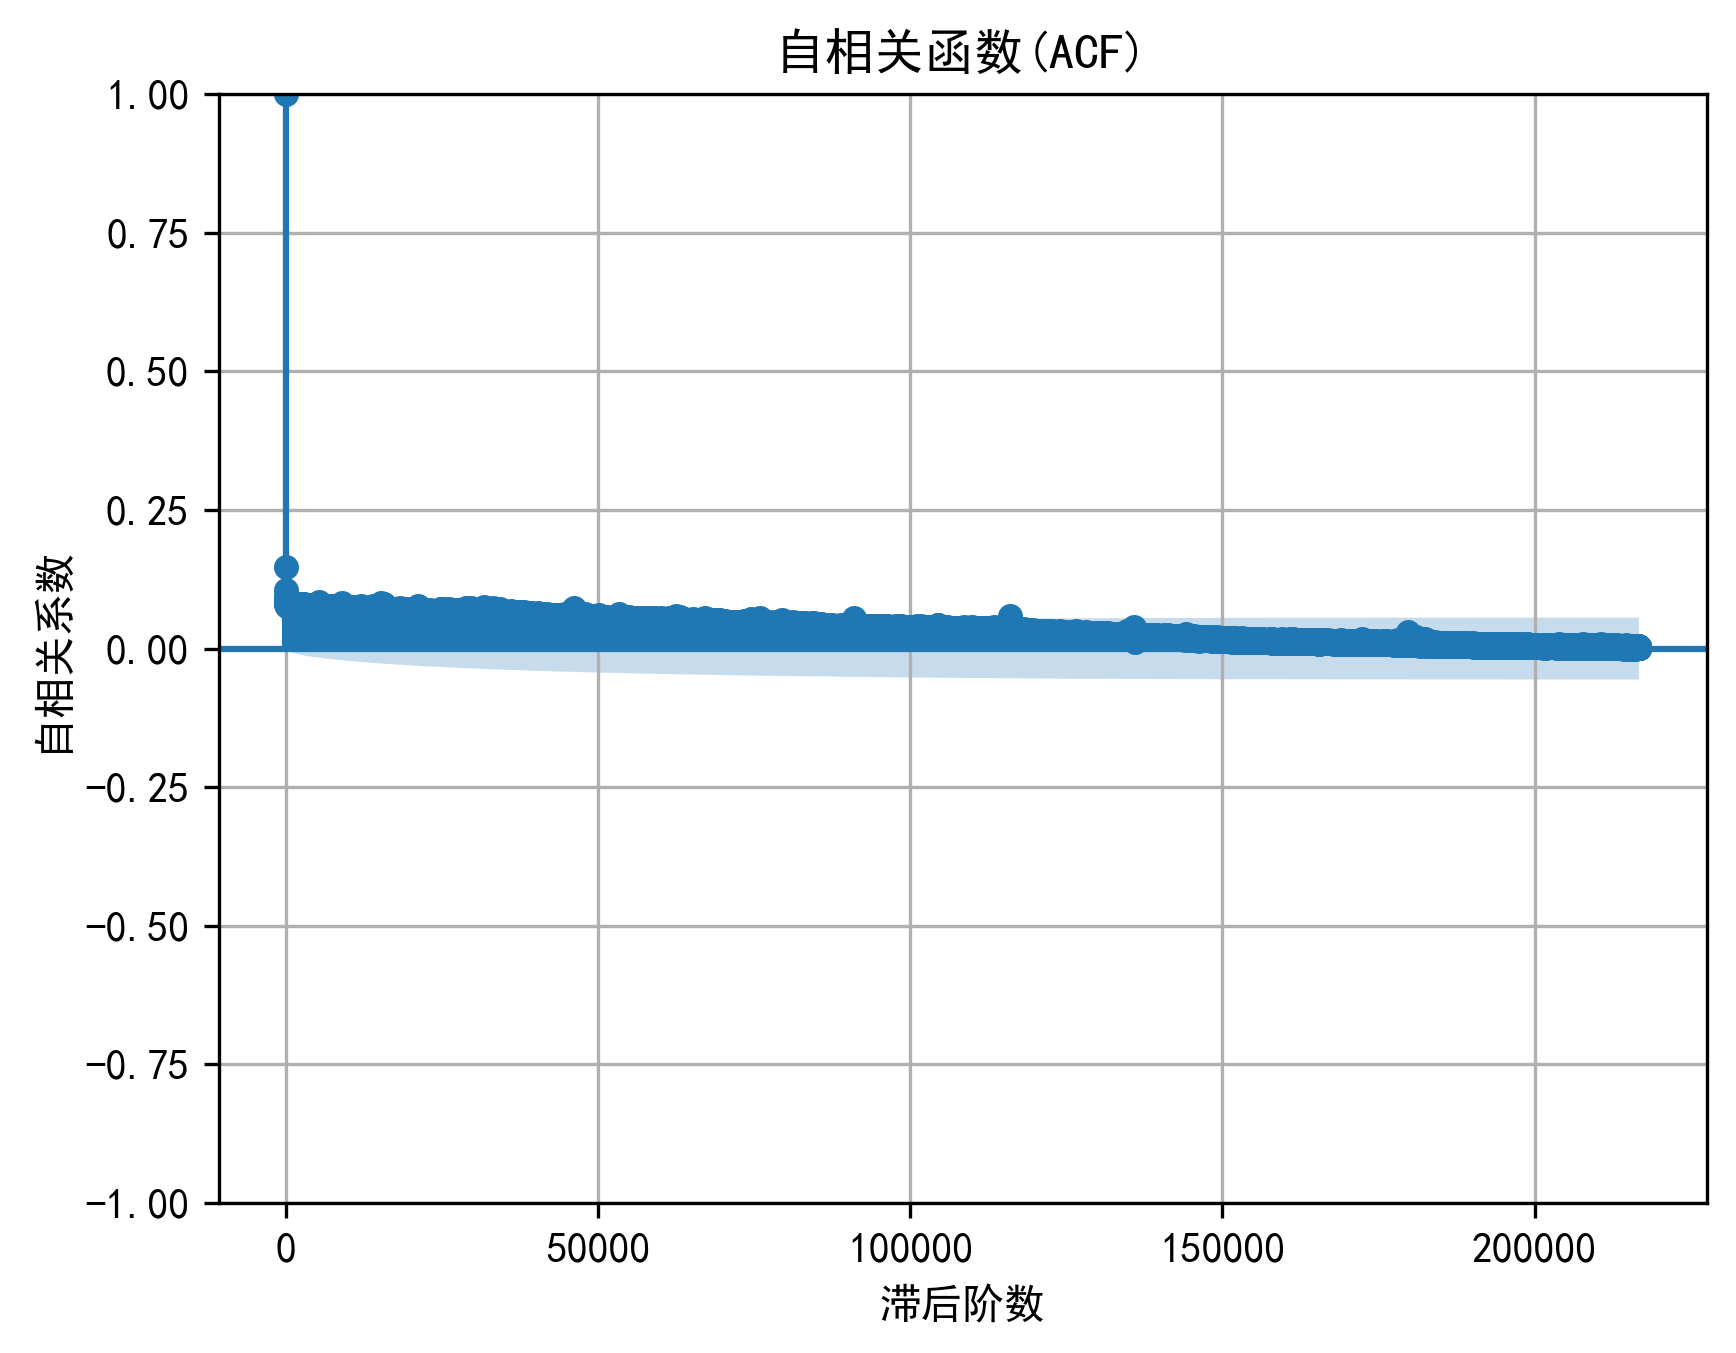
\includegraphics[width=0.7\textwidth]{calc_ACF/ACF_plot.png}
    \caption{总销量自相关函数(ACF)分析结果}
    \label{fig:acf}
\end{figure}
\textit{局部放大后图像}
\begin{figure}[H]
    \centering
    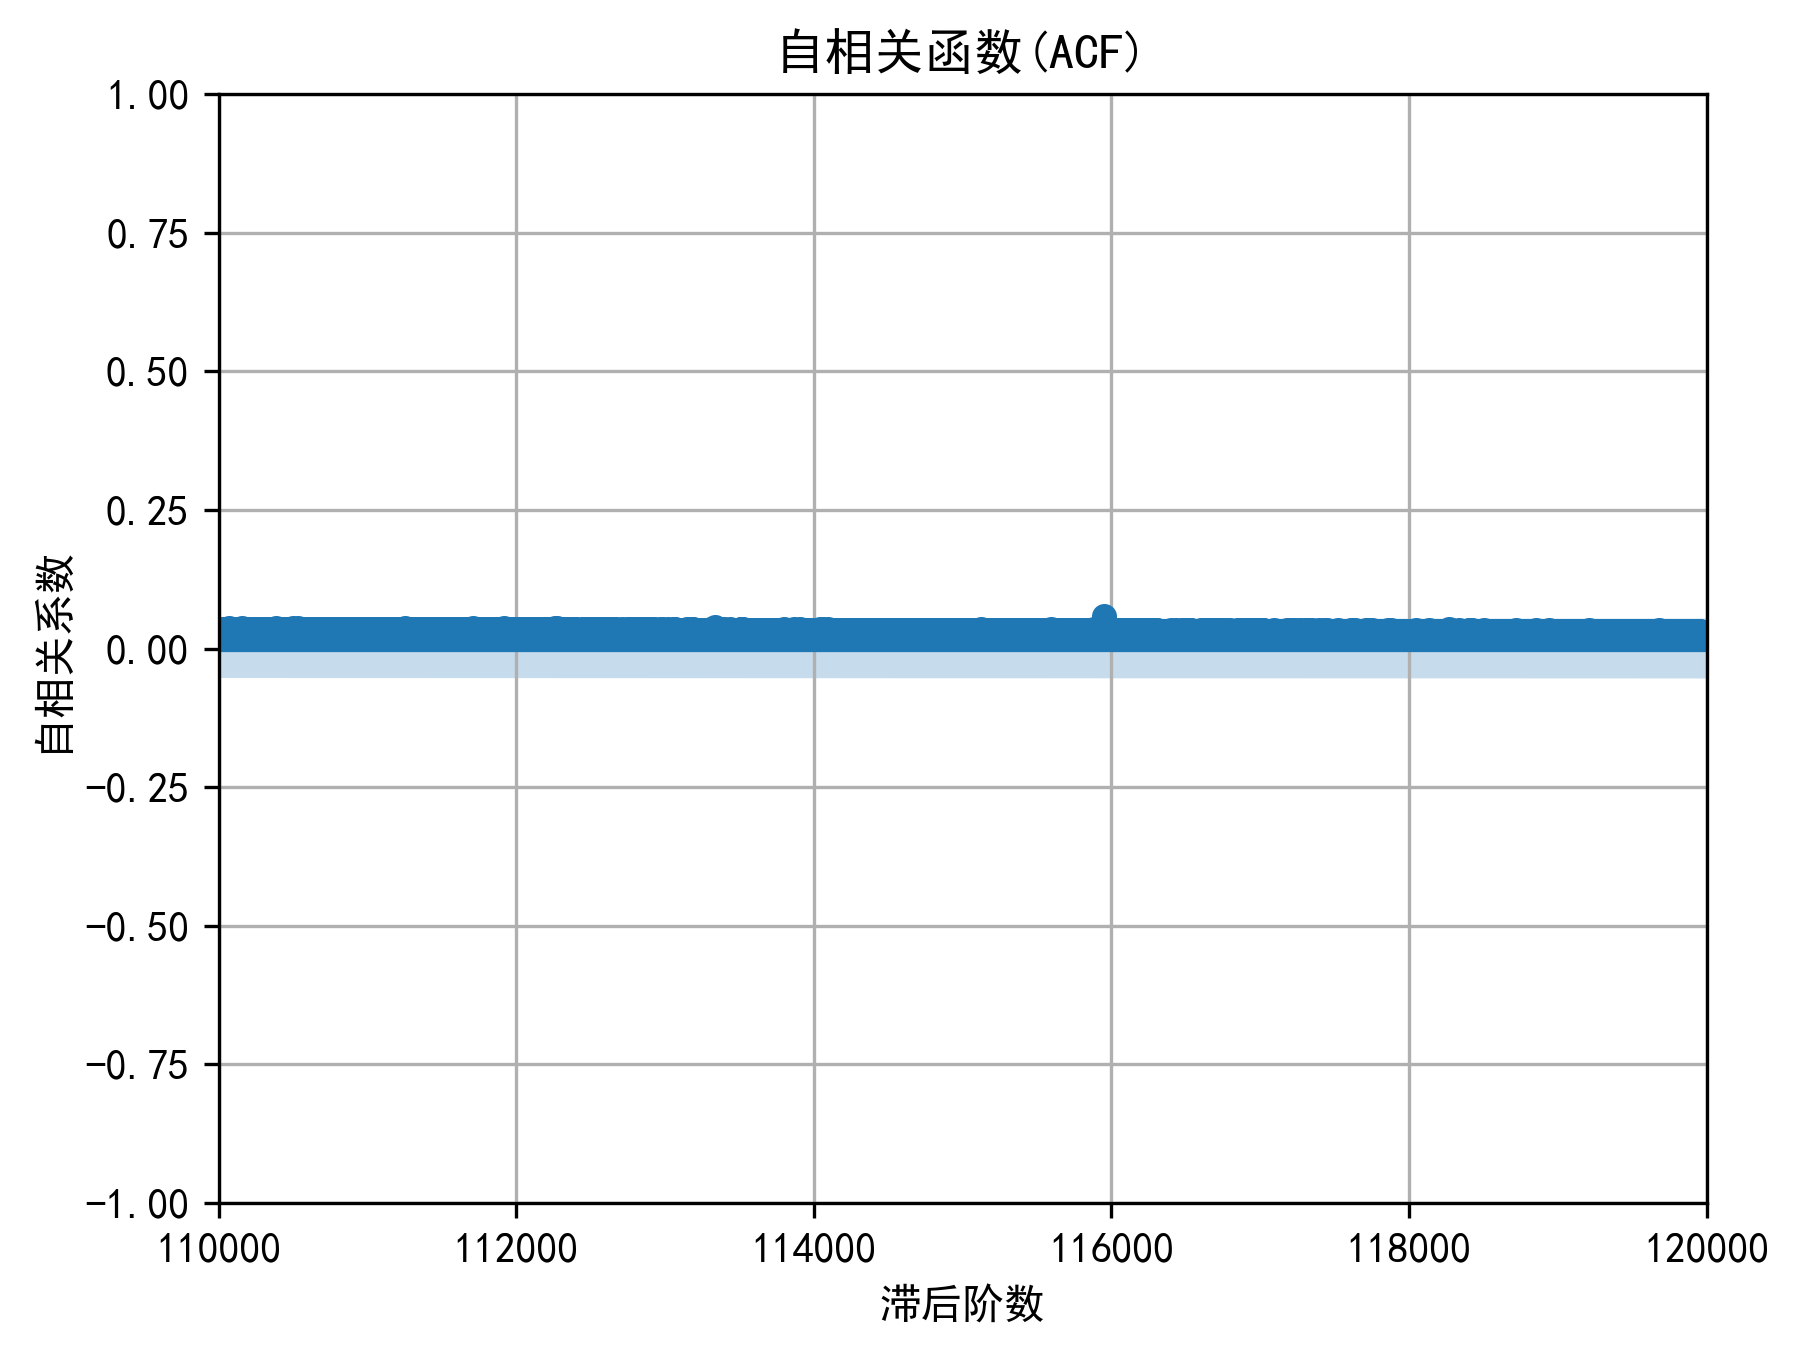
\includegraphics[width=0.7\textwidth]{calc_ACF/ACF_plot_zoomed.png}
    \caption{总销量自相关函数(ACF)分析结果(局部放大)}
    \label{fig:acf_zoomed}
\end{figure}
得到在短的滞后阶段内,总销售量随时间变化呈现出明显的周期性,但在长远的时间周期上,销售总量呈现出较为稳定的特点,比较符合经济学和生活中的常识。接下来我们对日销售量数据进行时间分布规律的分析,得到各蔬菜品类的销售量随时间变化的趋势图,
如图所示:
%这里要有至少3张图

\textit{商品定价分布规律模型}

计算各蔬菜品类的偏相关系数
\subsection{问题二模型求解}

\subsection{问题三模型求解}

\subsection{问题四模型求解}


%\section{模型检验}

\section{模型优点和展望}
\subsection{模型优点分析}
\begin{itemize}
    \item \textbf{问题一(关系分析):} 本文在分析蔬菜品类间的关系时,不仅采用了传统的相关性分析方法,还从“时间分布规律”、“定价分布规律”以及“品类间销量分布规律”三个角度进行系统性建模。特别地,通过引入偏相关系数,
    有效剔除了宏观因素对销量相关性的干扰,更加准确地揭示了各品类间的内在联系。同时,利用ACF(自相关系数)方法对销量的周期性进行分析,充分体现了时间序列分析的科学性和严谨性。

    \item \textbf{问题二(优化模型):} 针对补货与定价决策,模型将损耗率直接纳入单位成本的计算,提出
    \[
    \text{单位销售成本} = \frac{\text{预测批发价格}}{1 - \text{损耗率}}
    \]
    的计算方式,较传统的损耗处理方法更为精确。销售量与定价关系采用经济学中经典的双对数模型
    \[
    \ln(\text{销售量}) = \beta_0 + \beta_1 \ln(\text{销售价格})
    \]
    进行拟合,理论基础扎实,参数解释明确。

    \item \textbf{问题三(约束优化):} 针对实际业务需求,模型在连续线性规划的基础上,进一步引入多重约束条件,将问题转化为分段连续或混合整数规划模型,能够更好地适应实际补货与定价的复杂场景。
\end{itemize}
\newpage

\subsection{缺点与改进方向}
\begin{itemize}
    \item \textbf{部分假设和参数选择略显武断,需补充论证:} 在问题二的模型约束条件中,本研究采用最大销售量不超过历史最高的120\%  这是一个合理的约束,但这只是基于行业惯性和常识做出的限制,仍不够科学性、合理性,在查阅参考文献后,
    发现采用FP-Growth算法更为合理精确。

    \item \textbf{模型复杂度:} 在问题三中,模型的复杂度较高,可能导致求解时间较长。未来可以考虑使用启发式算法或元启发式算法(如遗传算法、粒子群优化等)来加速求解过程。

    \item \textbf{外部因素影响:} 模型未充分考虑外部因素(如天气、节假日等)对蔬菜销售的影响。未来可以通过引入更多的外部变量,增强模型的适应性和预测能力。
\end{itemize}
\end{document}